\chapter{Investigation of Visualization Tools using a Feature Classification Scheme}
\label{chap:Tools}

%single-task tool vs generic tool\cite{Brachman1996}
\section{Scalability in visualization tools}
Besides of the visualization technique itself the visualization tool influences the visual scalability in limiting how many datarows can be fetched in each visualization, the way the tool offers advanced visualization techniques and the interaction and analytical methods. Qlik Sense limits the initial fetch to 10.000 but gives the opportunity to fetch more data if needed. 
%Definition which tool meant: Tools can be divided into BI Tools, Analytic Tools, Visualization Tools and Custom Tools\cite{Schnell2014}.
%Difference Data Minining and Visual Analytics: First generate new knowledge and then visualiza vs. visualize and generate new knowledge

In this section we analyze selected visualization tools in business and their ability to analyze large time-oriented data. Therefore, we developed a classification scheme which is based on the collected success criteria of chapter 3. \\*
As discussed in chapter 3 visualization tools need to provide scalable visualization techniques or the ability to extend the tool with custom visualizations. Moreover, Interaction and distortion techniques are necessary to improve scalability and analytical methods to reduce the amount of data and 


Even though the selection of the tools is not exhaustive, we believe that the reviewed products represent the state-of-the art and provide the table of different tools which was used for chosing the remaining 5 tools in the appendix.
\subsection{The Classification Scheme}
The tools basis of assessment is the classification scheme which is devided into 3 \todo{maybe 4: Layout?} subsections: \textit{Analytical Techniques, Visualization Techniques, Interaction Techniques}. 
Each section contains success criteria which are necessary to display large time-oriented data. To rank the tools in the respecting category we developed the following success criteria score(SCS):

\begin{table}[th]
	\centering
	\caption[criteria]{Succes Criteria Score}
	\label{Succes Criteria Score}
	\begin{tabu}{cl}
	\toprule
	Points & Criteria\\
	\midrule
	4 & Native support by tool\\
	3 & Extension exists, but installation necessary \\
	2 & Extension can be programmed in a popular programming language (R,Javascript,Java) \\
	1 & Extension can be programmed, but in a tool-specific programming language \\
	0 & No support by tool\\
	\bottomrule
	\end{tabu}
\end{table}

\begin{figure}[H]
    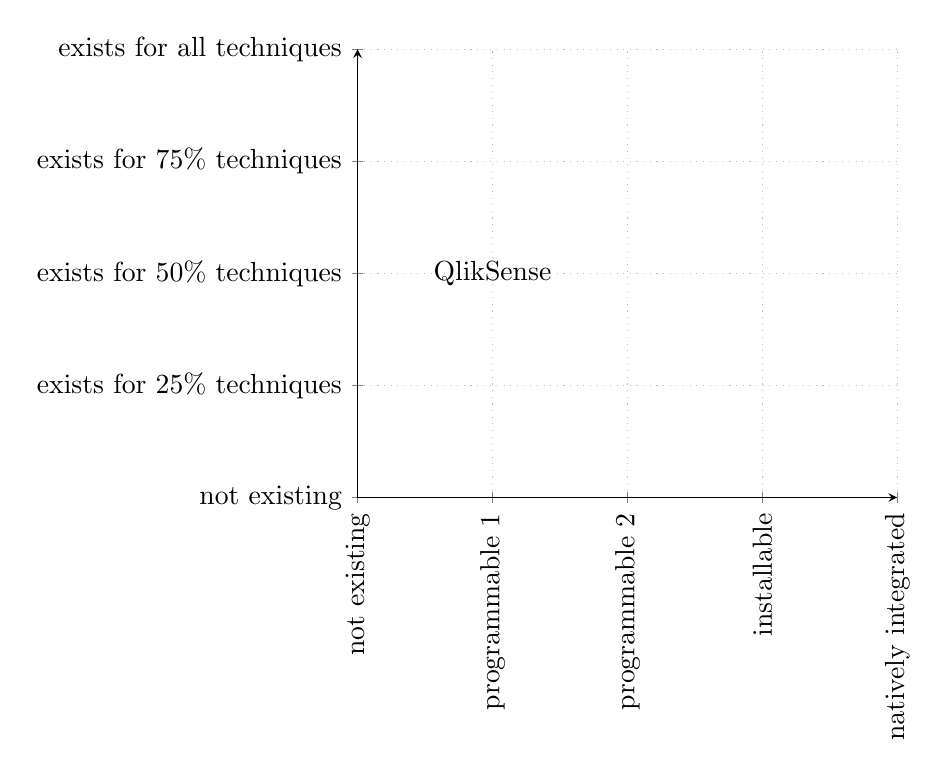
\begin{tikzpicture} 
        \begin{axis}[
         axis y line     = left,
              axis x line     = bottom,
        grid,
        grid style = {color=gray!50, dotted},
        xticklabels={,not existing, programmable 1, programmable 2, installable, natively integrated},
        xticklabel style={rotate=90},
        yticklabels={,not existing, exists for 25\% techniques, exists for 50\% techniques, exists for 75\% techniques, exists for all techniques},
        xmin       = 0, xmax = 4,
        ymin       = 0, ymax = 4,
        ]
        \node at (axis cs: 1,2)   {QlikSense};
        \end{axis}
    \end{tikzpicture}
    \caption{Success Criteria Scale} \label{classification}
\end{figure}

\subsection{Selection of Tools}
Advanced Data Visualization in business context requires software that is able to scale visualization in an "effective manner"\cite{Russom2011}. Offering advanced visualization techniques, parameterization, interaction and analytical methods such as data abstraction\cite{Tegarden1999,Aigner2011,Eick2002,Zhanga} are core functions of ADV software. Based on the Magic Quadrant for Business Intelligence and Analytics Platforms\cite{Parenteau2016} Qlik, Tableau and Microsoft are the leading visionaries of BI Vendors. \cite{ITCentralStation} as a crowdsourcing recommendation platform for BI tools ranked Tableau, Qlik, Oracle, Microsoft Power BI and IBM Cognos on the first five places.
\textbf{The Role of APIs}
Commercial software tends to need more time for the development and integration of advanced visualization for large data\cite{Zhanga, Simon2014}. To bridge the gap, vendors started to offer a bunch of APIs to create and integrate visualizations.
% data load for BigData: 
\textbf{Software not included in this work}
As the goal of this work is to compare software tools %alternative: provide a market overview
for Visual Analytics in business and time-oriented data we focus on Business Intelligence and Analytics software. Furthermore, the software needs visualization features, the ability to present time-dependent data. Software with one of the following items is intentionally not considered: 
\begin{enumerate}
    \item Software that only presents one-dimensional data. 
    \item Software that \todo{write reasons why Tools are not considered}
\end{enumerate}

\subsection{Qlik Sense}
Qliktech was founded in 1993 with the goal to "mimic how the brain works."\cite{qlikHistory}. They offer five products(Qlik Sense, Qlik Sense Cloud, QlikView, QlikView NPrinting, Qlik DataMarket) and the Qlik Analytics platform. Qlik Sense 1.0 was released in September 2014 for visual analytics. 
It offers functions such as Smart Data Load which allows to load large data from different data sources.
\subsubsection*{Analytics}
For analytics Qlik Sense support \text{Visual Data Preparation}: showing data tables as bubbles and connecting them by dragging and dropping them. Moreover, the user can create calculated fields\cite{qlikCalculated}.

\subsubsection*{Visualization Techniques}
Qlik Sense offers 8 built-in visualization techniques: bar charts, line charts, pie charts, scatterplots, treemap, maps, combi charts and gauge charts. If an additional technique is wanted the user can build a visualization extension with \textit{javascript} and \textit{QEXT} files\cite{qlikWorkbench}. Qlik Sense provides an extension template which supports the user in writing its extensions. However, the user needs to know javascript and html\cite{qlikVisExtensions}. Moreover, the Qlik Community offers ...\todo{anzahl an visualisierungen einfügen}
\textbf{Aggregation}: In the field of aggregation Qlik Sense offers data aggregation for one chart type: the scatterplot. Hereby, large data is aggregated by aggregation markers (squares) which represents the data point density by the color. The darker the square the denser the data\cite{qlikScatter}. 

\subsubsection*{Interaction}
To allow a focus + context view Qlik Sense offers navigational maps\cite{beard1990navigational},.
As a built-in-function Qlik Sense offers a navigational slider which shows a miniature version of the whole data set\cite{beard1990navigational}. 
Filters can be applied by making selections in the visualization\cite{qlikSheet}, the time range can be limited by zooming inside the visualization\cite{qlikTime} and all views then are adapted to the current selection. Thus, Qlik Sense offers Brushing + Linking. An edditional linking-feature are \textit{master items}\cite{qlikChangeData}, which allow the user to change properties for all master items at once.
For details the user can search Qlik Sense with Smart Search in which the dimensions, measures and metadata is searched and visualizations ,tables and KPIs are displayed\cite{qlikSmart}.  

\subsection{Tableau}
\subsubsection*{Visualization Techniques}
\textbf{Automatic Recommendation} partially is achieved with the function \textbf{Show Me}\cite{tableauShowme}. Tableau analyzes the given fields and recommends one of the implemented visualization technique. Hereby, Tableau is restricted to the known visualization techniques. 

\subsection{Power BI}
Microsoft Power Bi came alive in ...\todo{datum einfügen}. It offers 15 different visualization techniques. 

\subsubsection*{Visualization Techniques}
Microsoft Power BI offers 8 built-in visualization techniques: 15 different visualization techniques. Moreover, the Power BI visuals gallery offers 75 visualization apps. To build custom visualization apps the user needs to write \textit{TypeScript} or \textit{R}.
\textbf{Aggregation}: In the field of aggregation Qlik Sense offers data aggregation for one chart type: the scatterplot. Hereby, large data is aggregated by aggregation markers (squares) which represents the data point density by the color. The darker the square the denser the data\cite{qlikScatter}. 
\textbf{Aggregation}: Power BI offers one way to aggregate: calculated fields.
\subsubsection*{Interaction}
With cross-highlighting Power BI included brushing and linking in the tool\cite{powerbiInteract}, it offers filter functions. The focus mode enables the user to have a detailed view on the visualization. In focus mode the visualization will expand to full screen.  

\subsection{R}
R is a free and opensource language for statistical computing and graphics. Its modular structure consisting of many packages makes R highly extendable\cite{R}. Some packages enable the user to do analytics with R, others support different visualization techniques. Usually those packages also support interaction except the user additionally uses other libraries such as plot\_ly() or Shiny. Both of them are frameworks which combine R graphics with interaction techniques. Besides of that some packages offer interaction techniques, e.g. dygraphs(), while others do not. Thus, our classification scheme is only valid combined with specific packages.
There exists many packages which treat time-series data, e.g. \textit{zoo} and \textit{dygraphs} treat time-series. Large data sets are handled in \textit{bigvis}.
\subsubsection*{Analytics}
Out of the five tools R has the most extensive offer of analytical methods for time-series data. It is possible to detect patterns such as outliers with tsoutliers\cite{Chen1993} and clusters with tsclust\cite{Manso2015}, do advanced analytics with tswge\cite{tswge} and forecasting with zra\cite{zra}.
\subsubsection*{Visualization Techniques}
R supports standard visualization such as histograms, line charts and scatter plots. Advanced visualization techniques for large data sets 
\textbf{Aggregation}\\*
In the maps-package R offers the possibility to adjust the resolution with the parameter resolution. Resolution 0 maps the whole database whereas a higher resolution collapes data points within the resolution to one single point. This option allows to aggregate data and to only show the perceptual important points (PIP).
The bigvis and the hexbin package implement binning to condense large datasets\cite{Wickham2013}.
\textbf{Pixel-oriented} Time Series are visualized with mvtsplot\cite{mvtsplot}. This package allows to compare multivariate time-series data.
\subsubsection*{Interaction}
Plot\_ly()\cite{plotly} supports a brushing function with drill-down.
Shiny supports panning and zooming as well as linking and brushing.
Linked views are supported by plot\_ly() with and without shiny. 
Fish-eye views are implemented in the fisheyeR() package. 
The time range can be decreased by limiting the data range inside the code.
Animation can be achieved by using plot\_ly() and ggploty(). Moreover, plot\_ly() offers linked animated views.
\textit{Dygraphs} includes also navigational sliders called Range Selector, panning and zooming and brushing of data items.

\subsubsection{Conclusion}
Deck.gl offers a new way to present large datasets. WebBased, GPU-rendering with WebGL, programming in javascript. However, right now Deck.gl focuses on spatial data and requires programming skills. 